\documentclass[a4paper,oneside,12pt]{extreport}

\usepackage{mmap}
\usepackage[T2A]{fontenc}
\usepackage[utf8]{inputenc}
\usepackage[english,russian]{babel}


% Текст отчёта следует печатать, соблюдая следующие размеры полей:
% левое — 30 мм, правое — 15 мм, верхнее и нижнее — 20 мм.
\usepackage[left=20mm, right=15mm, top=15mm, bottom=15mm]{geometry}

% \setlength{\parindent}{1.25cm} % Абзацный отступ

\usepackage{setspace}
%\onehalfspacing % Полуторный интервал

\frenchspacing % Равномерные пробелы
\usepackage{indentfirst} % Красная строка

\usepackage{microtype}
\sloppy

\usepackage{titlesec}
\titlespacing*{\chapter}{0pt}{-30pt}{8pt}
\titlespacing*{\section}{\parindent}{*4}{*4}
\titlespacing*{\subsection}{\parindent}{*4}{*4}
\titleformat{\chapter}{\LARGE\bfseries}{\thechapter}{20pt}{\LARGE\bfseries}
\titleformat{\section}{\Large\bfseries}{\thesection}{40pt}{\Large\bfseries}

\usepackage{graphicx}
\usepackage{caption}

\usepackage[unicode,pdftex]{hyperref}
\hypersetup{hidelinks}

%% title begin
\usepackage{wrapfig}

\makeatletter
	\def\vhrulefill#1{\leavevmode\leaders\hrule\@height#1\hfill \kern\z@}
\makeatother
%% title end

%% begin code
\usepackage{listings}
\usepackage{xcolor}

\lstset{
	basicstyle=\footnotesize\ttfamily,
	breakatwhitespace=true,
	breaklines=true,
	commentstyle=\color{gray},
	frame=single,
	keywordstyle=\color{blue},
	stringstyle=\color{red},
	tabsize=8
}

\lstdefinestyle{lispinline}{
	frame=none,
	language=Lisp
}

\newcommand{\code}[1]{\texttt{#1}}
%% end code

%% begin theorem
\usepackage{amsthm}

\makeatletter
\newtheoremstyle{indented}
	{}% measure of space to leave above the theorem
	{}% measure of space to leave below the theorem
	{}% name of font to use in the body of the theorem
	{\parindent}% measure of space to indent
	{\bfseries}% name of head font
	{.}% punctuation between head and body
	{ }% space after theorem head; " " = normal interword space
	{}% header specification (empty for default)
\makeatother

\theoremstyle{indented}

\newtheorem{definition}{Определение}[section]
\newtheorem{example}{Пример}[section]
\newtheorem{theorem}{Теорема}[section]
\newtheorem{task}{Задание}

\makeatletter
\DeclareRobustCommand\bfseriesitshape{%
	\not@math@alphabet\itshapebfseries\relax
	\fontseries\bfdefault
	\fontshape\itdefault
	\selectfont
}
\makeatother

\DeclareTextFontCommand{\textbfit}{\bfseriesitshape}
\DeclareTextFontCommand{\define}{\bfseriesitshape}
%% end theorem

%% begin columns
\usepackage{etoolbox,refcount}
\usepackage{multicol}

\newcounter{countitems}
\newcounter{nextitemizecount}
\newcommand{\setupcountitems}{%
	\stepcounter{nextitemizecount}%
	\setcounter{countitems}{0}%
	\preto\item{\stepcounter{countitems}}%
}
\makeatletter
\newcommand{\computecountitems}{%
	\edef\@currentlabel{\number\c@countitems}%
	\label{countitems@\number\numexpr\value{nextitemizecount}-1\relax}%
}
\newcommand{\nextitemizecount}{%
	\getrefnumber{countitems@\number\c@nextitemizecount}%
}
\newcommand{\previtemizecount}{%
	\getrefnumber{countitems@\number\numexpr\value{nextitemizecount}-1\relax}%
}
\makeatother
\newenvironment{AutoMultiColItemize}{%
	\ifnumcomp{\nextitemizecount}{>}{3}{\begin{multicols}{2}}{}%
		\setupcountitems\begin{itemize}}%
		{\end{itemize}%
		\unskip\computecountitems\ifnumcomp{\previtemizecount}{>}{3}{\end{multicols}}{}}
\makeatother
\newenvironment{AutoMultiColEnumerate}{%
	\ifnumcomp{\nextitemizecount}{>}{3}{\begin{multicols}{2}}{}%
		\setupcountitems\begin{enumerate}}%
		{\end{enumerate}%
		\unskip\computecountitems\ifnumcomp{\previtemizecount}{>}{3}{\end{multicols}}{}}
%% end columns

	
\usepackage{amsmath}

\begin{document}

\begin{titlepage}
	{\large % 14pt instead of 12pt
	\onehalfspacing
	\centering

	\begin{wrapfigure}[7]{l}{0.14\linewidth}
		\vspace{3mm}
		\hspace{-10mm}
		
\includegraphics[width=\linewidth]{img/b_logo}
		% \includegraphics[width=0.93\linewidth]{inc/img/bmstu-logo}
	\end{wrapfigure}
	{\singlespacing \footnotesize \bfseries Министерство науки и высшего образования Российской Федерации\\Федеральное государственное бюджетное образовательное учреждение\\высшего образования\\<<Московский государственный технический университет\\имени Н.~Э.~Баумана\\ (национальный исследовательский университет)>>\\(МГТУ им. Н.~Э.~Баумана)\\}

	\vspace{-2.2mm}
	\vhrulefill{0.9mm}\\
	\vspace{-7.5mm}
	\vhrulefill{0.2mm}\\
	\vspace{2mm}

	{\doublespacing \small \raggedright ФАКУЛЬТЕТ \hspace{5mm} \underline{«Информатика и системы управления»}\\
	КАФЕДРА \hspace{10mm} \underline{«Программное обеспечение ЭВМ и информационные технологии»}\\}

	\vspace{20mm}

	\begin{center}
		\noindent\begin{minipage}{1.2\textwidth}\centering
			\textbf{ОТЧЕТ ПО ЛАБОРАТОРНОЙ РАБОТЕ №4}\newline
			\textbf{По курсу: "Моделирование"}\newline\newline\newline
		\end{minipage}
	\end{center}

	\vspace{20mm}

	\noindent ~~Тема \underline{~~~~~Программно-алгоритмическая реализация моделей~~~~~~~~~~~~~~~~~~~~~}\newline
	\underline{~~~~~~~~~~~~~~на основе дифференциальных уравнений в~~~~~~~~~~~~~~~~~~~~~~~~~~~~~~~~~}\newline
	\underline{~~~~~~~частных производных с краевыми условиями II и III рода.~~~~~~~~~~~~~~~~~~}\newline
	\noindent ~~Группа \underline{~~~~~~~~~~~~~~~~~~~~~~~~~~~~~~~~~~~ИУ7-63Б~~~~~~~~~~~~~~~~~~~~~~~~~~~~~~~~~~~~~~~~~~~~~~~~~}\newline
	\noindent ~~Студент \underline{~~~~~~~~~~~~~~~~~~~~~~~~~~~~Сукочева А.~~~~~~~~~~~~~~~~~~~~~~~~~~~~~~~~~~~~~~~~~~~~~~~~~~}\newline
	\noindent ~~Преподаватель \underline{~~~~~~~~~~~~~~~~~Градов В.М.~~~~~~~~~~~~~~~~~~~~~~~~~~~~~~~~~~~~~~~~~~~~~~~~~~~}\newline


	\begin{center}
		\vfill
		Москва~---~\the\year
		~г.
	\end{center}
	}



\end{titlepage}

\setcounter{page}{2}

\section{Постановка задачи}
\textbf{Цель работы}. 
Получение навыков разработки алгоритмов решения смешанной краевой
задачи при реализации моделей, построенных на квазилинейном уравнении
параболического типа.

\subsection{Исходные данные}

Задана математическая модель.

Уравнение для функции $T(x,t)$

\begin{equation}
	c(T) \frac{\partial T}{\partial t} = \frac{\partial}{\partial x} (k(T) \frac{\partial T}{\partial x}) - \frac{2}{R}\alpha(x)T + \frac{2T_{0}}{R}\alpha(x)
\end{equation}\\

Краевые условия:

\begin{equation}
	\begin{cases} t = 0, T(x, 0) = T_{0}
	\\ x = 0, - k(T(0)) \frac{\partial T}{\partial x} = F_{0}
	\\ x = l, - k(T(l)) \frac{\partial T}{\partial x} = \alpha_{N} (T(l) - T_{0})
	\end{cases}
\end{equation}\\

В обозначениях уравнения лекции:

\begin{equation}
	p(x) = \frac{2}{R} \alpha(x)
\end{equation}

\begin{equation}
	f(u) = f(x) = \frac{2T_{0}}{R}\alpha(x)
\end{equation}

Разностная схема с разностным краевым условие при $x = 0$:

\begin{equation*}
	(\frac{h}{8} \buildrel\,\,\frown\over{c_{\frac{1}{2}}} + \frac{h}{4} \buildrel\,\,\frown\over{c_{0}} + \buildrel\,\,\frown\over{X_{\frac{1}{2}}} \frac{\tau}{h} + \frac{\tau h}{8} p_{\frac{1}{2}} + \frac{\tau h}{4}p_{0}) \buildrel\,\,\frown\over{y_{0}} + (\frac{h}{8} \buildrel\,\,\frown\over{c_{\frac{1}{2}}} - \buildrel\,\,\frown\over{X_{\frac{1}{2}}} \frac{\tau}{h} + \frac{\tau h}{8} p_\frac{1}{2}) \buildrel\,\,\frown\over{y_{1}} = 
\end{equation*}

\begin{equation}
	= \frac{h}{8} \buildrel\,\,\frown\over{c_{\frac{1}{2}}} (y_{0} + y_{1}) + \frac{h}{4} \buildrel\,\,\frown\over{c_{0}} y_{0} + \buildrel\,\,\frown\over{F}\tau + \frac{\tau h}{4} (\buildrel\,\,\frown\over{f_{\frac{1}{2}}} + \buildrel\,\,\frown\over{c_{0}})
\end{equation}\\

При получении разностного аналога краевого условия при $x = l$ учесть, что поток:

\begin{equation}
	F_{N} = \alpha{N}(y_{N} - T_{0}), F_{N - \frac{1}{2}} = X_{N - \frac{1}{2}} \frac{y_{N - 1} - y_{N}}{h}
\end{equation}

Заданы начальные параметры:\\

\begin{itemize}
	\item $k(T) = a_{1}(b_{1} + c_{1}T^{m_{1}})$, Вт/см K
	\item $c(T) = a_{2} + b_{2} T^{m_{2}} - \frac{c_{2}}{T^2}$, Дж/c$m^3$ K
	\item $a_{1} = 0.0134, b_{1} = 1, c_{1} = 4.35 \cdot 10^{-4}, m_{1} = 1$
	\item $a_{2} = 2.049, b_{2} = 0.563 \cdot 10^{-3}, c_{2} = 0.528 \cdot 10^{5}, m_{2} = 1$
	\item $\alpha(x) = \frac{c}{x - d}, \alpha_{0} = 0.05$ Вт/с$m^2$ K, $\alpha_{N} = 0.01$ Вт/c$m^2$ K
	\item $l = 10$ см
	\item $T_{0} = 300K$
	\item $R$ = 0.5 см
	\item $F(t) = 50$ Вт/с$m^2$
\end{itemize}


\newpage 
\section{Реализация}

\begin{lstlisting}[]
using System;
using System.Collections.Generic;

namespace src
{
	class Conditions
	{
		static public double[] GetLeftConditions(List<double> T)
		{
			double c_plus = Functions.ApproximationPlus(Functions.c, T[0], Constants.t);
			double k_plus = Functions.ApproximationPlus(Functions.k, T[0], Constants.t);

			double K0 = Constants.h / 8 * c_plus + Constants.h / 4 * Functions.c(T[0]) + Constants.t / Constants.h * k_plus + 
					Constants.t * Constants.h / 8 * Functions.p(Constants.h / 2) + Constants.t * Constants.h / 4 * Functions.p(0);

			double M0 = Constants.h / 8 * c_plus - Constants.t / Constants.h * k_plus + Constants.t * Constants.h / 8 * Functions.p(Constants.h / 2);

			double P0 = Constants.h / 8 * c_plus * (T[0] + T[1]) + Constants.h / 4 * Functions.c(T[0]) * T[0] + 
					Constants.F0 * Constants.t + Constants.t * Constants.h / 8 * (3 * Functions.f(0) + Functions.f(Constants.h));

			double[] result = { K0, M0, P0 };
			return result;
		}

		static public double[] GetRightConditions(List<double> T)
		{
			double c_minus = Functions.ApproximationMinus(Functions.c, T[T.Count - 1], Constants.t);
			double k_minus = Functions.ApproximationMinus(Functions.k, T[T.Count - 1], Constants.t);

			double KN = Constants.h / 8 * c_minus + Constants.h / 4 * Functions.c(T[T.Count - 1]) + Constants.t / Constants.h * k_minus + 
					Constants.t * Constants.alphaN + Constants.t * Constants.h / 8 * Functions.p(Constants.l - Constants.h / 2) + 
					Constants.t * Constants.h / 4 * Functions.p(Constants.l);

			double MN = Constants.h / 8 * c_minus - Constants.t / Constants.h * k_minus + 
					Constants.t * Constants.h / 8 * Functions.p(Constants.l - Constants.h / 2);

			double PN = Constants.h / 8 * c_minus * (T[T.Count - 1] + T[T.Count - 2]) + Constants.h / 4 * Functions.c(T[T.Count - 1]) * T[T.Count - 1] + 
					Constants.t * Constants.alphaN * Constants.T0 + Constants.t * Constants.h / 4 * (Functions.f(Constants.l) + Functions.f(Constants.l - Constants.h / 2));

			double[] result = {KN, MN, PN};
			return result;
		}

		static public List<double> GetNewT(List<double> T)
		{
			double[] cond = GetLeftConditions(T);
			double K0 = cond[0], M0 = cond[1], P0 = cond[2];

			cond = GetRightConditions(T);
			double KN = cond[0], MN = cond[1], PN = cond[2];

			List<double> xi = new List<double>();
			xi.Add(0); xi.Add(-M0 / K0);

			List<double> eta = new List<double>();
			eta.Add(0); eta.Add(P0 / K0);

			double x = Constants.h, Tn, denominator, next_xi, next_eta;
			int n = 1;

			while (x + Constants.h < Constants.l)
			{
				Tn = T[n];
				denominator = (Functions.B(x, Tn) - Functions.A(Tn) * xi[n]);

				next_xi = Functions.D(Tn) / denominator;
				next_eta = (Functions.F(x, Tn) + Functions.A(Tn) * eta[n]) / denominator;

				xi.Add(next_xi);
				eta.Add(next_eta);

				n++;
				x += Constants.h;
			} 

			List<double> T_new = new List<double>();
			for (int i = 0; i < n + 1; i++)
				T_new.Add(0);
			
			T_new[n] = (PN - MN * eta[n]) / (KN + MN * xi[n]);
			
			for (int i = n - 1; i > -1; i--)
				T_new[i] = xi[i + 1] * T_new[i + 1] + eta[i + 1];

			return T_new;
		}
	}
}
\end{lstlisting}

\begin{lstlisting}[]
	namespace src
	{
		public static class Constants
		{
			public const double a1 = 0.0134;
			public const double b1 = 1;
			public const double c1 = 4.35e-4;
			public const double m1 = 1;
			public const double a2 = 2.049;
			public const double b2 = 0.563e-3;
			public const double c2 = 0.528e5;
			public const double m2 = 1;
			public const double alpha0 = 0.05;
			public const double alphaN = 0.01;
			public const double l = 10;
			public const double T0 = 300;
			public const double R = 0.5;
			public const double F0 = 50;
			public const double h = 1e-3;
			public const double t = 1;
			public const double eps = 1e-2;
		}
	}
	\end{lstlisting}

\begin{lstlisting}[]
using System;

namespace src
{
	class Functions
	{
		static public double k(double T)
		{
			return Constants.a1 * (Constants.b1 + Constants.c1 * Math.Pow(T, Constants.m1));
		}

		static public double c(double T)
		{
			return Constants.a2 + Constants.b2 * Math.Pow(T, Constants.m2) - (Constants.c2 / Math.Pow(T, 2));
		}
		
		static public double alpha(double x)
		{
			double d = (Constants.alphaN * Constants.l) / (Constants.alphaN - Constants.alpha0);
			double c = -Constants.alpha0 * d;
			return c / (x - d);
		}

		static public double p(double x)
		{
			return alpha(x) * 2 / Constants.R;
		}

		static public double f(double x)
		{
			return alpha(x) * 2 * Constants.T0 / Constants.R;
		}

		static public double ApproximationPlus(Func<double, double> f, double n, double step)
		{
			return (f(n) + f(n + step)) / 2;
		}

		static public double ApproximationMinus(Func<double, double> f, double n, double step)
		{
			return (f(n) + f(n - step)) / 2;
		}

		static public double A(double T)
		{
			return Constants.t / Constants.h * ApproximationMinus(k, T, Constants.t);
		}

		static public double D(double T)
		{
			return Constants.t / Constants.h * ApproximationPlus(k, T, Constants.t);
		}

		static public double B(double x, double T)
		{
			return A(T) + D(T) + Constants.h * c(T) + Constants.h * Constants.t * p(x);
		}

		static public double F(double x, double T)
		{
			return Constants.h * Constants.t * f(x) + T * Constants.h* c(T);
		}


	}
}
\end{lstlisting}

\begin{lstlisting}[]
using System;
using System.Collections.Generic;
using System.Linq;
using System.IO;

namespace src
{
	class Program
	{
		static void SaveData(List<double> res, string fileName)
		{
			FileStream file = new FileStream(fileName, FileMode.Create, FileAccess.Write);
			StreamWriter writer = new StreamWriter(file);

			foreach (var elem in res)
			{
				writer.WriteLine(elem);
			}

			writer.Close();
			file.Close();
		}

		static void Task()
		{
			List<double> T = Enumerable.Range(1, (int)(Constants.l / Constants.h) + 1).Select(x => (double)Constants.T0).ToList();
			List<double> TNew = Enumerable.Range(1, (int)(Constants.l / Constants.h) + 1).Select(x => 0d).ToList();
			List<double> TPrev = new List<double>();

			double currentMax = 1d, ti = 0;

			bool epsilonCondition = true;
			int file_i = 0;
			
			SaveData(T, $"results/data/task_1_{file_i++}.txt");

			while (epsilonCondition)
			{
				TPrev = T;
				currentMax = 1d;

				while (currentMax >= 1)
				{
					TNew = Conditions.GetNewT(T);
					currentMax = Math.Abs((T[0] - TNew[0]) / TNew[0]);

					var arr_d = T.Zip(TNew, (T_i, Tnew_i) => Math.Abs(T_i - Tnew_i) / Tnew_i);
					currentMax = arr_d.Max();

					TPrev = TNew;
				}

				SaveData(TNew, $"results/data/task_1_{file_i++}.txt");

				ti += Constants.t;

				epsilonCondition = false;
				int flag = T.Zip(TNew, (T_i, Tnew_i) => Math.Abs(T_i - Tnew_i) / Tnew_i).Count(elem => elem > Constants.eps);
				if (flag != 0)
					epsilonCondition = true;

				T = TNew;

				// List<double> ys = new List<double>();
				// for (double s = 0; s < Constants.l / 3d> ; s += 0.1)
				// {
				// 	Console.WriteLine(s);
				// 	ys.Add(TNew[(int)(s / Constants.h)]);
				// }
				// SaveData(ys, $"results/data/task_2_{file_i++}.txt");
			}
		}

		static void Main(string[] args)
		{
			// Output with point.
			System.Threading.Thread.CurrentThread.CurrentCulture = new System.Globalization.CultureInfo("en-US");
			Task();
		}
	}
}	
\end{lstlisting}

% \begin{lstlisting}[]
% \end{lstlisting}


\newpage 

\section{Экспериментальная часть}

\section*{Результаты работы программы}

\textbf{1. Представить разностный аналог краевого условия при $x = l$ и его краткий вывод интегро-интерполяционным методом.}\\


\textbf{2. График зависимости температуры $T(x, t_{m})$ от координаты $x$ при нескольких фкисированных значених времени $t_{m}$ при заданных выше параметрах. }\\

% \begin{figure}[ht!]
% 	\centering{
% 		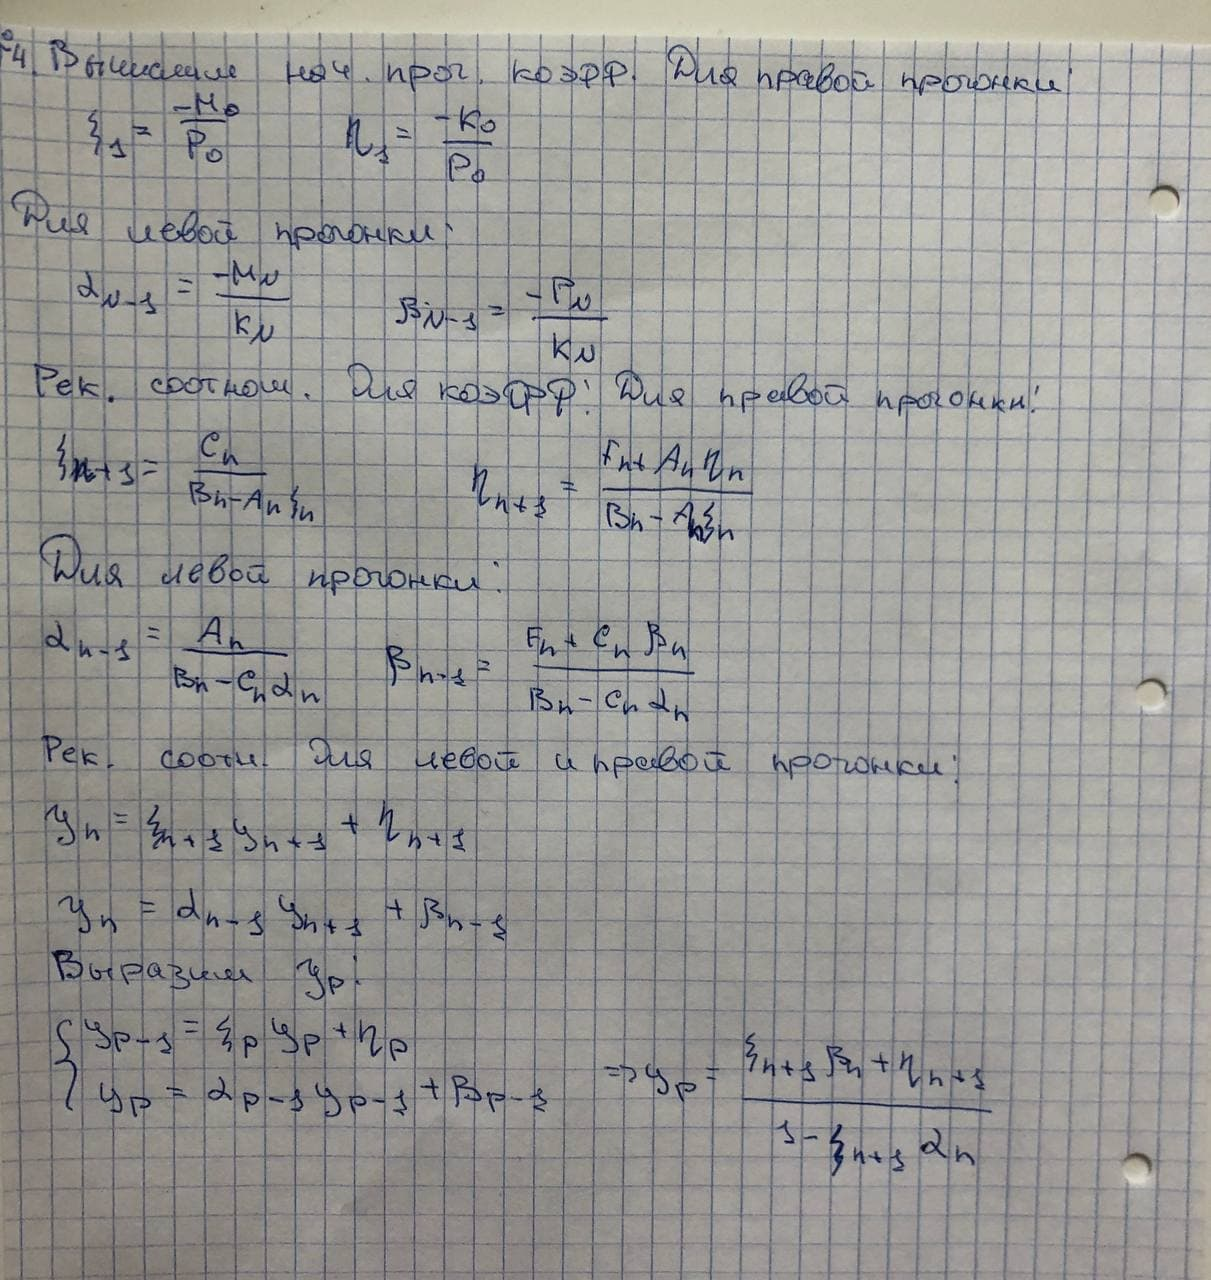
\includegraphics[width=0.7\textwidth]{img/v3.jpg}}
% \end{figure}

\end{document}